% **************************************************
% Document Class Definition
% **************************************************
\documentclass{mimosis}


% **************************************************
% Setup YOUR thesis document in this file !
% **************************************************
% !TEX root = my-thesis.tex


% **************************************************
% Files' Character Encoding
% **************************************************
\PassOptionsToPackage{utf8}{inputenc}
\usepackage{inputenc}


% **************************************************
% Information and Commands for Reuse
% **************************************************
\newcommand{\thesisTitle}{In-sensor Stochastic Computing Implementations and Comparative Analysis with \\ Conventional Digital Computing}
\newcommand{\thesisName}{DO LE DUY}
\newcommand{\thesisSubject}{Bachelor Thesis}
\newcommand{\thesisDate}{Feb 7, 2024}
\newcommand{\thesisVersion}{First Draft}


\newcommand{\thesisSupervisor}{Prof. Masanori Hashimoto}
\newcommand{\thesisSupervisorGroup}{Integrated Systems Engineering Laboratory}

\newcommand{\thesisUniversity}{\protect{Kyoto University}}
\newcommand{\thesisUniversitySchool}{School of Engineering}
\newcommand{\thesisUniversityDepartment}{Department of Electrical and Electronic Engineering}
\newcommand{\thesisUniversityGroup}{Integrated Systems Engineering Laboratory}


% **************************************************
% Fonts
% **************************************************
\usepackage{charter}
\usepackage[oldstyle,scale=0.7]{sourcecodepro}


% **************************************************
% Load and Configure Packages
% **************************************************
\usepackage[english]{babel} % babel system, adjust the language of the content
\usepackage{scrhack}


\setlength{\parindent}{0pt} % Remove para indent
\setstretch{1.2} % value for line spacing, use \setstretch{} 
\setlength{\parskip}{1em} % value for paragraph indentation

\usepackage{amsmath}

% Save the original \frac command in case it's needed
\let\oldfrac\frac
% Redefine \frac to be \dfrac
\renewcommand{\frac}[2]{\dfrac{#1}{#2}}


% Move figures to end of thesis
\usepackage[nomarkers]{endfloat}
% Redefine the separator between figures/tables
\renewcommand{\efloatseparator}{\vspace{1cm}}


% Adjust section titles formating
% \usepackage{titlesec}
% \titleformat{\section}
% {\normalfont\large\bfseries}{\thesection}{1em}{}
% \titleformat{\subsection}
% {\normalfont\normalsize\bfseries}{\thesubsection}{1em}{}

\usepackage[%
  colorlinks = true,
  citecolor  = RoyalBlue,
  linkcolor  = RoyalBlue,
  urlcolor   = RoyalBlue,
  ]{hyperref}

% Setup biblatex
\usepackage[%
  autocite     = plain,
  backend      = biber,
  doi          = true,
  url          = true,
  giveninits   = true,
  hyperref     = true,
  maxbibnames  = 99,
  maxcitenames = 99,
  sortcites    = true,
  style        = numeric,
  ]{biblatex}

% %%%%%%%%%%%%%%%%%%%%%%%%%%%%%%%%%%%%%%%%%%%%%%%%%%%%%%%%%%%%%%%%%%%%%%%%
% Some adjustments to make the bibliography more clean
%%%%%%%%%%%%%%%%%%%%%%%%%%%%%%%%%%%%%%%%%%%%%%%%%%%%%%%%%%%%%%%%%%%%%%%%
%
% The subsequent commands do the following:
%  - Removing the month field from the bibliography
%  - Fixing the Oxford commma
%  - Suppress the "in" for journal articles
%  - Remove the parentheses of the year in an article
%  - Delimit volume and issue of an article by a colon ":" instead of
%    a dot ""
%  - Use commas to separate the location of publishers from their name
%  - Remove the abbreviation for technical reports
%  - Display the label of bibliographic entries without brackets in the
%    bibliography
%  - Ensure that DOIs are followed by a non-breakable space
%  - Use hair spaces between initials of authors
%  - Make the font size of citations smaller
%  - Fixing ordinal numbers (1st, 2nd, 3rd, and so) on by using
%    superscripts

% Remove the month field from the bibliography. It does not serve a good
% purpose, I guess. And often, it cannot be used because the journals
% have some crazy issue policies.
\AtEveryBibitem{\clearfield{month}}
\AtEveryCitekey{\clearfield{month}}

% Fixing the Oxford comma. Not sure whether this is the proper solution.
% More information is available under [1] and [2].
%
% [1] http://tex.stackexchange.com/questions/97712/biblatex-apa-style-is-missing-a-comma-in-the-references-why
% [2] http://tex.stackexchange.com/questions/44048/use-et-al-in-biblatex-custom-style
%
\AtBeginBibliography{%
  \renewcommand*{\finalnamedelim}{%
    \ifthenelse{\value{listcount} > 2}{%
      \addcomma
      \addspace
      \bibstring{and}%
    }{%
      \addspace
      \bibstring{and}%
    }
  }
}

% Suppress "in" for journal articles. This is unnecessary in my opinion
% because the journal title is typeset in italics anyway.
\renewbibmacro{in:}{%
  \ifentrytype{article}
  {%
  }%
  % else
  {%
    \printtext{\bibstring{in}\intitlepunct}%
  }%
}

% Remove the parentheses for the year in an article. This removes a lot
% of undesired parentheses in the bibliography, thereby improving the
% readability. Moreover, it makes the look of the bibliography more
% consistent.
\renewbibmacro*{issue+date}{%
  \setunit{\addcomma\space}
    \iffieldundef{issue}
      {\usebibmacro{date}}
      {\printfield{issue}%
       \setunit*{\addspace}%
       \usebibmacro{date}}%
  \newunit}

% Delimit the volume and the number of an article by a colon instead of
% by a dot, which I consider to be more readable.
\renewbibmacro*{volume+number+eid}{%
  \printfield{volume}%
  \setunit*{\addcolon}%
  \printfield{number}%
  \setunit{\addcomma\space}%
  \printfield{eid}%
}

% Do not use a colon for the publisher location. Instead, connect
% publisher, location, and date via commas.
\renewbibmacro*{publisher+location+date}{%
  \printlist{publisher}%
  \setunit*{\addcomma\space}%
  \printlist{location}%
  \setunit*{\addcomma\space}%
  \usebibmacro{date}%
  \newunit%
}

% Ditto for other entry types.
\renewbibmacro*{organization+location+date}{%
  \printlist{location}%
  \setunit*{\addcomma\space}%
  \printlist{organization}%
  \setunit*{\addcomma\space}%
  \usebibmacro{date}%
  \newunit%
}

% Display the label of a bibliographic entry in bare style, without any
% brackets. I like this more than the default.
%
% Note that this is *really* the proper and official way of doing this.
\DeclareFieldFormat{labelnumberwidth}{#1\adddot}

% Ensure that DOIs are followed by a non-breakable space.
\DeclareFieldFormat{doi}{%
  \mkbibacro{DOI}\addcolon\addnbspace
    \ifhyperref
      {\href{http://dx.doi.org/#1}{\nolinkurl{#1}}}
      %
      {\nolinkurl{#1}}
}

% Use proper hair spaces between initials as suggested by Bringhurst and
% others.
\renewcommand*\bibinitdelim {\addnbthinspace}
\renewcommand*\bibnamedelima{\addnbthinspace}
\renewcommand*\bibnamedelimb{\addnbthinspace}
\renewcommand*\bibnamedelimi{\addnbthinspace}

% Make the font size of citations smaller. Depending on your selected
% font, you might not need this.
\usepackage{relsize}
\renewcommand*{\citesetup}{%
  \biburlsetup
  \relsize{-.5}%
}

\DeclareLanguageMapping{english}{english-mimosis}

% Make hyperlinks extend to the author name if `\textcite` is being used
% instead of another cite command.

\DeclareFieldFormat{citehyperref}{%
  % Need this to avoid nested links
  \DeclareFieldAlias{bibhyperref}{noformat}%
  \bibhyperref{#1}%
}

\DeclareFieldFormat{textcitehyperref}{%
  % Need this to avoid nested links
  \DeclareFieldAlias{bibhyperref}{noformat}%
  \bibhyperref{%
    #1%
    \ifbool{cbx:parens}
      {\bibcloseparen\global\boolfalse{cbx:parens}}
      {}%
    }%
}

\savebibmacro{cite}
\savebibmacro{textcite}

\renewbibmacro*{cite}{%
  \printtext[citehyperref]{%
    \restorebibmacro{cite}%
    \usebibmacro{cite}}%
}

\renewbibmacro*{textcite}{%
  \ifboolexpr{
    ( not test {\iffieldundef{prenote}} and
      test {\ifnumequal{\value{citecount}}{1}} )
    or
    ( not test {\iffieldundef{postnote}} and
      test {\ifnumequal{\value{citecount}}{\value{citetotal}}} )
  }%
  {\DeclareFieldAlias{textcitehyperref}{noformat}}
  {}%
  \printtext[textcitehyperref]{%
    \restorebibmacro{textcite}%
    \usebibmacro{textcite}}%
}

\addbibresource{Thesis.bib}




% **************************************************
% Document CONTENT
% **************************************************
\begin{document}

% uncomment the following command to fill up pages with
% whitespace instead of aligning the first and last lines
% of a page (see \raggedbottom vs. \flushbottom)
%\raggedbottom

% --------------------------
% rename document parts
% --------------------------

% > set short label names for floating environments figure and table
%\renewcaptionname{ngerman}{\figurename}{Abb.}
%\renewcaptionname{ngerman}{\tablename}{Tab.}
\renewcaptionname{english}{\figurename}{Fig.}
\renewcaptionname{english}{\tablename}{Tab.}



% --------------------------
% Front matter
% --------------------------
\pagenumbering{roman}			% roman page numbing (invisible for empty page style)
\pagestyle{empty}				% no header or footers
% !TEX root = ../my-thesis.tex
%
% % ------------------------------------  --> cover title page
% \begin{titlepage}
% 	\pdfbookmark[0]{Cover}{Cover}
% 	\flushright
% 	\hfill
% 	\vfill
% 	{\LARGE\thesisTitle \par}
% 	\rule[5pt]{\textwidth}{.4pt} \par
% 	{\Large\thesisName}
% 	\vfill
% 	\textit{\large\thesisDate} \\
% 	Version: \thesisVersion
% \end{titlepage}


% ------------------------------------  --> main title page
\begin{titlepage}
	\centering

	{\Large \thesisUniversity} \\[4mm]
	
\includegraphics[width=2cm]{gfx/E-C.pdf} \\[2mm]
	\textsf{\thesisUniversitySchool} \\
	\textsf{\thesisUniversityDepartment} \\ [30mm]


	{\large \thesisSubject} \\[5mm]
	{\LARGE \textbf{\thesisTitle} \\[10mm]}
	{\Large \thesisName} \\

	\hspace*{15pt}

	\emph{Thesis submitted to the undergraduate degree program in the Electrical and Electronic Engineering Department, Undergraduate School of Engineering at Kyoto University in partial fulfillment of the requirements for the degree of \\ Bachelor of Engineering.} \\ [15mm]


	Supervised by \thesisSupervisor \\[3mm]
	\thesisUniversityGroup \\[3mm]
	
	\thesisDate \\

\end{titlepage}


% ------------------------------------  --> lower title back for single page layout
\hfill
\vfill
{
	\small
	\textbf{\thesisName} \\
	\textit{\thesisTitle} \\
	\thesisSubject, \thesisDate \\
	Supervised by \thesisSupervisor \\[1.5em]
	\textbf{\thesisUniversity} \\

	\thesisUniversityDepartment \\
	\thesisUniversitySchool \\
}		% INCLUDE: all titlepages
\pagestyle{plain}				% display just page numbers

\setcounter{tocdepth}{2}		% define depth of toc
\tableofcontents				% display table of contents
\cleardoublepage 

% --------------------------
% Body matter
% --------------------------
\pagenumbering{arabic}			% arabic page numbering
\setcounter{page}{1}			% set page counter

\clearpairofpagestyles % Reset header and footer style
\pagestyle{scrheadings}
\ohead{\leftmark}
\ofoot[\pagemark]{\pagemark} 

\automark[chapter]{chapter}

% !TEX root = ../my-thesis.tex
%
\chapter{Introduction}
\label{sec:intro}

\section{Research Background}
\label{sec:intro:bg}

The development in computing, often encapsulated by Moore's Law, has continually pushed the boundaries of processing power and miniaturization. However, as we approach the physical limits of silicon-based technologies, the quest for more energy-efficient computing paradigms has become paramount. Conventional digital computing, despite its widespread adoption and success, faces significant challenges in sustaining energy efficiency gains.

In this context, novel computing methods that significantly deviate from traditional von Neumann architectures have been investigated to further progress toward reducing computational complexity, power consumption, and physical footprint.

Stochastic computing (SC), which processes data using random bit streams and conventional digital logic, is one such solution. It diverges significantly from traditional binary computing by using extremely simple hardware to manipulate data in serial bitstreams. While many fundamental concepts of stochastic computing were already developed in the 1960s, the progress was stalled in the next several decades due to its perceived impracticality in favor of traditional digital approaches. 

However, interest has been reignited in SC in the last decade for advantage in implementing several computing processes as well as potential compatibility with neuromorphic computing paradigms. The development of SC has shifted from the basic theories of fundamental elements to more complex applications like artificial neural networks (ANNs) as research is addressing fundamental challenges to make SC more broadly applicable. These include designing stochastic architectures that are power efficient and exploring the hardware design space for such architectures.

Properties such as inherent fault tolerance and a lower hardware cost while maintaining performance have been observed to be a key advantage of stochastic computing, such as illustrated in applications like image segmentation. However, the steep trade-off between precision and latency as well as the overhead hardware cost of stochastic bitstream generation remained roadblocks to efficient SC hardware. 

Incorporating SC within the edge computing domain presents a
promising frontier. In-sensor computing, which integrates processing
capabilities directly within sensors, aligns well with the
minimalistic nature of SC. 

As data from external sources are processed directly
at the point of collection, in-sensor approaches could reduce latency in decision-making
processes as well as minimizes the energy consumption and bandwidth requirements
typically associated with the process of analog-to-digital conversion and data transmission to centralized processing units.
These edge systems could perform complex tasks like real-time analytics, edge AI
computations, and immediate decision-making, essential for applications in IoT,
autonomous systems, environmental monitoring, and healthcare. 

The synergy of SC with in-sensor computing could lead to a new generation of smart sensors capable of sophisticated data processing with minimal footprint. The challenge lies
in optimizing the SC design to maintain accuracy and efficiency while
capitalizing on the benefits of localized data processing.


\section{Research Purpose}
\label{sec:intro:motivation}

The purpose of this research is to explore the in-sensor implementation of Stochastic Computing (SC) and to conduct a comparative analysis with conventional digital computing. Instead of assuming binary format as inputs to the system and adopting digital-to-stochastic converters, we will consider input signals from sensors developed for optimal usage in stochastic computing. Thus, this work aims to answer two fundamental questions: how certain edge applications can be implemented efficiently using SC, and whether the benefits of SC outweigh those of conventional digital computing.

To achieve these objectives, we will employ a variety of tools and methodologies. Cocotb and Ikarus will be used for the verification of Register-Transfer Level (RTL) designs using Python, ensuring accurate performance of our stochastic computing implementations for ASIC designs in selected applications. Xilinx Vivado will be utilized to synthesize and analyze our stochastic computing designs on FPGA platforms. This will allow us to assess performance, power consumption, and area utilization of SC implementations in a comparative context. Finally, Gem5, a modular platform for computer-system architecture research, will be employed to simulate these applications on conventional digital computing platforms, focusing on CPU-based systems.

In this thesis, Chapter 1 introduces the research background and purpose, setting the stage for a detailed exploration of Stochastic Computing (SC). Chapter 2 delves into the technical aspects of SC, including various bitstream representations, computing elements, and architectures. Chapter 3 discusses practical applications of SC in fields like image processing and machine learning. Chapter 4 outlines the methodologies used, including the specific versions and configurations of utilized tools including Vivado and Gem5. Chapter 5 presents the results and comparative analysis between SC and conventional digital computing. The thesis concludes with Chapter 6, offering conclusions and directions for our future research.




% !TEX root = ../my-thesis.tex
%
\chapter{Review}
\label{sec:review}

\section{Stochastic Computing: Fundamental Concepts}
\label{sec:review:sec1}

Stochastic Computing (SC) circuits represent a paradigm shift in computational method, enabling arithmetic functions with minimal logic gates. This is achieved by  encoding values into patterns of random bit sequences, a stochastic number. For example, the number $\frac{1}{3}$ can be shown as a series of bits like $0, 0, 1, 0, 1, 0$, where the number of 1's is one-third of the total.

In this framework, each bit in the series is considered a random variable, $X$, following a Bernoulli distribution with a probability $p_X$ of being 1. $X$ is also used to denote the stochastic number that is collectively represented by the series, commonly referred to as bit sequences or bitstreams. As big letters i.e $X$ denote stochastic numbers, $p_X$ denote probabilities encoded in the bitstreams, we use small letters i.e $x$ for the actual values linked to stochastic numbers.

There are two major ways to represent actual values as stochastic number. For a positive real parameter $M$, the unipolar encoding $X$ could represent a non-negative real number $x$ such that $0 \leq x \leq M$ by having $p_X = \frac{x}{M} $. On the other hand, the bipolar encoding $X$ could represent a real number $x$ such that $-M \leq x \leq M$ by having $p_X  = \frac{x}{2M} + \frac{1}{2}$.

We could also interpret that in unipolar encoding, zeros in the bitstream are weighted as 0 and ones are weighted as +1, thus limits unipolar encoding to the positive range [0, M]. On the other hand, bipolar encoding weights zeros as -1 and ones as +1, allowing the range [-M, +M]. Therefore, depend on the format, we would configure the counter circuit of Stochastic-to-Digital Converters (SDC) differently to return the correct value in binary format. 


\subsection {Correlation}

The correlation between bitstream is a major consideration when designing SC circuit. Most SC circuits operate best with a specific input SN correlation. The correlation level between bitstreams is assessed using the stochastic computing correlation (SCC). An SCC value of +1.0 signifies maximum positive correlation, -1.0 indicates maximum negative correlation, and 0.0 implies the bitstreams are uncorrelated. 

For example, the circuit for multiplying with AND Gate for unipolar encoding or XOR Gate for bipolar encoding works best with uncorrelated bitstream. Accuracy in computation improves as the correlation of input bitstreams approaches the optimal SCC value.

By contrast, some operations would be possible with positive correlation, while for some it would not be necessary to take correlation into consideration. 

\section{Bitstream Representations of Values}
\label{sec:review:sec2}

The accuracy of a stochastic number gets better with a longer sequence, a
feature called progressive precision. At least 11 bits are needed to encode the
probability $5/11$; at least 16 bits are needed to encode $5/16$. Since the
bits are random, you often need a much longer sequence to get close to the exact
average you want. However, in real-life, stochastic numbers often aren't perfect
because the bits can be influenced by previous bits in the sequence. This can
make the computations less efficient or accurate There are two types of
stochastic numbers: `ideal,' where each bit is independent and doesn't rely on
the previous bits, and `non-ideal,' where the bits are influenced by their
history in the sequence.

\subsection{Bitstream Generation}

\subsection {Linear-Feedback Shift Registers}

A popular method for generating random numbers in stochastic computing (SC) is
using a linear-feedback shift register (LFSR). An N-bit LFSR consists of N
flip-flops and XOR gates, forming a feedback loop. With N bits, there are
$ (2^ N - 1)$ potential combinations leaving zero. As a maximal LFSR
cycles through these  $(2 N - 1 )$ numbers in a pseudo-random order, it can generate approximately  $2^ {n-1}$ bits long stochastic bitstream. 

To ensure multiple bitstreams remaining uncorelated, LFSRs may be configured with different seeds. Each LFSR would go through the same sequence but at different stages. Circuits like 
isolators, synchronizers, desynchronizers, decorrelators, and regenerators can alter the correlation of existing stochastic numbers (SNs).

Cost-saving measures include sharing schemes with memory components like flip-flops to vary the stages of the same LFSR.

\subsection {Low-Discrepancy Sequences}

Additionally, low discrepancy sequences like Van der Corput, Halton, and Sobol are also considered for sequence generators (SNGs) due to their equidistribution properties.

These sequences distribute more evenly compared to
pseudo-random sequences generated by LFSRs, leading to faster convergence in
probability calculations. The van der Corput sequence, a one-dimensional LD
sequence, is created by reversing the digits of natural numbers in a specific
base. The Halton sequence extends this to higher dimensions using co-prime bases.
The Sobol' sequence, a base-2 sequence, is also notable for its distinct,
infinite-length properties.


\subsection{Deterministic Bitstream}

Stochastic representations could be considered uniform representations, the value is encoded in
the fraction of time the signal is high. 


\begin{figure}[htb]
	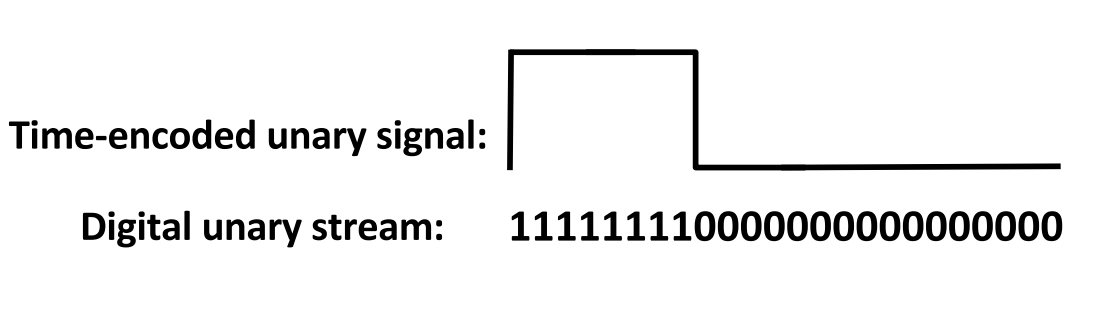
\includegraphics[width=12cm]{gfx/Time-encode signal.png}
	\caption{Time-based bitstream}
	\label{fig:system:example1}
\end{figure}



\section{Stochastic Computing Elements}
\label{sec:review:sec3}


In stochastic computing, certain computational elements can be effectively implemented using fundamental gates with minimal footprint. This efficiency stems from the fundamental properties of these gates in relation to probabilistic operations:

$\bullet$ NOT Gate (Complement): $p_Q  = 1 - p_X $ \\
$\bullet$ AND Gate (Joint Probability): $p_Q  = p_X p_Y $ \\
$\bullet$ OR Gate (Union of Independent Events): $p_Q  = p_X + p_Y - p_Xp_Y $

\begin{figure}[htb]
	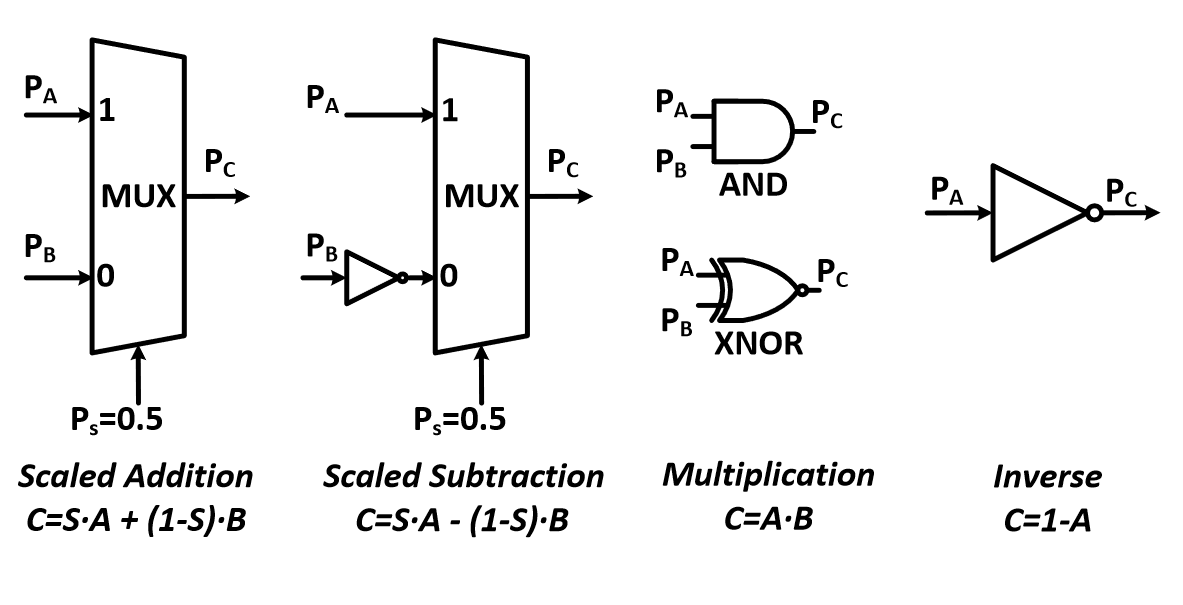
\includegraphics[width=12cm]{gfx/SC elements.png}
	\caption{Stochastic computational elements}
	\label{fig:system:example1}
\end{figure}

While the operation on bitstream is universal for every circuit, the actual calculations when mapped to real value depend on initial encoding. For example, operations with NOT Gates  return equivalent real-valued output that can be expressed as $q = -x$ in bipolar encoding and $q = M-x$ in unipolar encoding. 

\subsection{Multiplication}

In the context of unipolar encoding, multiplication can be executed using an AND gate. When two bitstreams representing stochastic numbers $X $ and $Y $ pass through an AND gate, the resultant stochastic number (SN) $Q $ encodes the probability $p_Q  = p_X p_Y $. With scale constant of the output 
being  $M_Q  = M_X M_Y$ whereas $M_X, M_Y$ are input scale constants, the relationship becomes $$p_Q  = \frac{x}{M_X}\frac{y}{M_Y} = \frac{xy}{M_Q } \rightarrow \frac{q}{M_Q } .$$

For bipolar encoding, multiplication is implemented using an XNOR gate. The output SN $Q $ in this case encodes the probability $p_Q  = 1 - p_X (1-p_Y) - (1-p_X) p_Y = 1 - p_X - p_Y + 2p_Xp_Y$. Substituting the bipolar mappings for $x, y, q$, we have: 

$$\begin{aligned} 
\frac{q}{2M_Q} + \frac{1}{2} &= 1 - \frac{x}{2M_X} - \frac{1}{2} - \frac{Y}{2M_Y} - \frac{1}{2} + 2\left(\frac{x}{2M_X} + \frac{1}{2}\right) \left(\frac{y}{2M_Y} + \frac{1}{2}\right) \\
\implies \frac{q}{M_Q} &= \frac{x}{M_X} \frac{y}{M_Y}
\end{aligned}$$

Thus, for inputs $x $ and $y $, and output $q $, with $M_Q = M_X \cdot M_Y$ the relationship simplifies to $q = a \cdot b $, interpreting the XNOR gate as a multiplier in bipolar contexts.

Stochastic computing's implementation of multiplication, utilizing only a single gate, is one of its major advantages over conventional circuits. However, for accurate results, the bitstreams involved in multiplication must be uncorrelated (i.e., independent).

\subsection{Scaled Addition/Subtraction}

Besides multiplication, scaled addition can be effectively implemented in both bipolar and unipolar formats using a multiplexer (MUX). The select input $S $ of the MUX, a unipolar stochastic number with $M = 1 $, acts as a weighting factor ranging from 0 to 1. The result is expressed with the following equation: $$p_Q  = (1 - p_S) \cdot p_X + p_S \cdot p_B .$$ 

Thus, having $p_S = 0.5$ effectively averaging the probabilities of the two inputs. As inverse operation is only available in bipolar encoding, scaled subtraction is exclusive to this format and achieved through a combination of a MUX and a NOT gate. 

We also note that only the correlation between the select signal and inputs affects output accuracy, while the correlation between inputs does not.

\subsection{Operations using Correlated Bitstream}

On the other hand, correlated bitstreams also have advantages by enabling efficient implementation of maximum, minimum, and absolute difference functions using basic logic gates. An OR Gate outputs the maximum value when fed with two correlated bitstreams, as
it favors high values present in either stream. An AND Gate produces the minimum value from correlated inputs, as it outputs high only when
both inputs are high. A XOR Gate calculates the absolute
difference between correlated streams, outputting high values when the inputs
differ, reflecting the magnitude of the difference.


\begin{figure}[htb]
	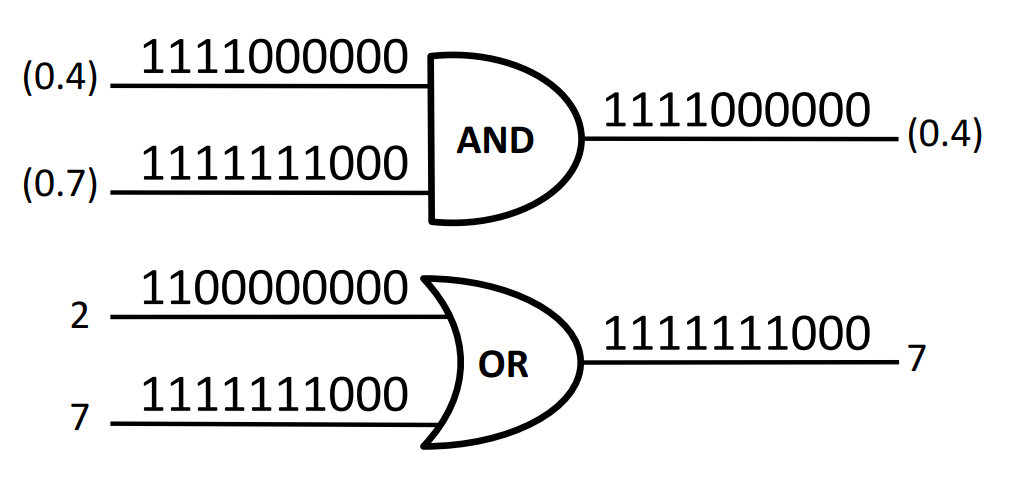
\includegraphics[width=12cm]{gfx/maxmin.png}
	\caption{Computational elements with correlated bitstream}
	\label{fig:system:example1}
\end{figure}

A generic linear state transition diagram


\section{Function Approximations with Sequential Logic}
\label{sec:review:sec4}

Combinational logic in stochastic computing is primarily effective for implementing polynomial functions that map the unit interval to itself. 
Techniques based on Bernstein polynomials have been proposed for approximating
polynomials using only multiplexers (MUX) and full-adders, but this method
is limited to the unipolar format. Non-polynomial functions can be approximated using methods like MacLaurin expansions; however, this approach struggles with highly nonlinear functions like exponentiation and tanh.

Given the limitations of combinational logic in handling more complex functions, the use of sequential logic with Finite State Machines (FSMs) has been explored. FSMs allow for the execution of sophisticated functions that are beyond the scope of combinational logic, broadening the application range of stochastic computing.

The state machine shown in Fig. - contains a set of
states, $S_0, S_1, \dots , S_{N-1}$, arranged in a linear form as a saturating counter. It has a total of N states, where $N$ is a positive integer. We usually set $N=2^K$, where $K$ is also a positive integer, since the maximum number of states can be implemented by $K$ D-Flip-Flops (DFFs) is $2^K . X$ is the input of this state machine. The output $Y$ of this state machine is only determined by the current state. We assume that the input $X$ is a Bernoulli sequence (i.e., a stochastic bit stream).

The system can be modeled as a time-homogeneous irreducible and aperiodic Markov chain and will have one single stable hyperstate. We define the probability that each bit in the input stream $X$ is one to be $P_X$, the probability that each bit in the corresponding output stream $Y$ is one to be $P_Y$, and in the steady state the probability that the current state is $S_i(0 \leq i \leq N-1)$ under the input probability $P_X$ to be $P_{i\left(P_X\right)}$. The individual state probability $P_{i\left(P_X\right)}$ in the hyperstate must sum to unity, and the probability of transitioning from state $S_{i-1}$ to state $S_i$ must equal the probability of transitioning from state $S_i$ to state $S_{i-1}$. Thus, we have
$$
\begin{gathered}
P_{i\left(P_X\right)} \cdot\left(1-P_X\right)=P_{i-1\left(P_X\right)} \cdot P_X, \\
\sum_{i=0}^{N-1} P_{i\left(P_X\right)}=1, \\
P_Y=\sum_{i=0}^{N-1} s_i \cdot P_{i\left(P_X\right)},
\end{gathered}
$$
where $s_i$ only has two choices of values, 0 or 1 , and specifies the output $Y$ of the system when the current state is $S_i$, i.e., if the current state is $S_i$, then the output $Y=s_i$. $P_{i\left(P_X\right)}$ can be computed as follows,
$$
P_{i\left(P_X\right)}=\frac{\left(\frac{P_X}{1-P_X}\right)^i}{\sum_{j=0}^{N-1}\left(\frac{P_X}{1-P_X}\right)^j} .
$$


\begin{figure}[htb]
	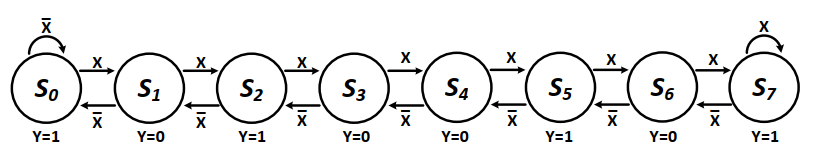
\includegraphics[width=12cm]{gfx/Generic LSM.png}
	\caption{A generic linear state transition diagram}
	\label{fig:system:example1}
\end{figure}

Designs haven been proposed to implement various function with different output schemes for $s_i$. One of the earliest is the Stochastic Tanh Function (STanh). 

\subsection{Stochastic Tanh Function (STanh)}



The output $s_i$ is configured as follows,
$$
s_i= \begin{cases}0, & 0 \leq i \leq \frac{N}{2}-1 \\ 1, & \frac{N}{2} \leq i \leq N-1\end{cases}
$$

\begin{figure}[htb]
	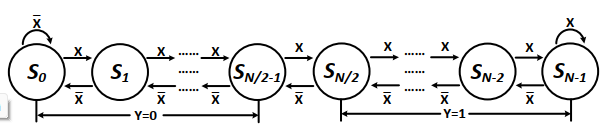
\includegraphics[width=12cm]{gfx/tanhlsm.png}
	\caption{State transition diagram of the STanh Function}
	\label{fig:system:example1}
\end{figure}

The stochastic tanh (STanh) circuit (Figure ) could approximates a tanh function:
$$
y \approx \frac{e^{\frac{N}{2} x}-e^{-\frac{N}{2} x}}{e^{\frac{N}{2} x}+e^{-\frac{N}{2} x}},
$$
where $x$ is the bipolar encoding of the input bit stream $X$ and $y$ is also the bipolar encoding of the output bit stream $Y$. 

Proof: We have
$$
P_Y=\sum_{i=N / 2}^{N-1} P_{i\left(P_X\right)}
$$

If we substitute $P_{i\left(P_X\right)}$, we have
$$
\begin{aligned}
P_Y & =\frac{\sum_{i=N / 2}^{N-1}\left(\frac{P_X}{1-P_X}\right)^i}{\sum_{k=0}^{N-1}\left(\frac{P_X}{1-P_X}\right)^k}=\frac{\left(\frac{P_X}{1-P_X}\right)^{\frac{N}{2}}-\left(\frac{P_X}{1-P_X}\right)^N}{1-\left(\frac{P_X}{1-P_X}\right)^N} \\
& =\frac{\left(\frac{P_X}{1-P_X}\right)^{\frac{N}{2}} \cdot\left(1-\left(\frac{P_X}{1-P_X}\right)^{\frac{N}{2}}\right)}{\left(1+\left(\frac{P_X}{1-P_X}\right)^{\frac{N}{2}}\right) \cdot\left(1-\left(\frac{P_X}{1-P_X}\right)^{\frac{N}{2}}\right)} \\
& =\frac{\left(\frac{P_X}{1-P_X}\right)^{\frac{N}{2}}}{1+\left(\frac{P_X}{1-P_X}\right)^{\frac{N}{2}}} .
\end{aligned}
$$

If we substitute $P_X$ and $P_Y$ in with their corresponding bipolar coding format $x$ and $y$, we have
$$
\frac{y+1}{2}=\frac{\left(\frac{1+x}{1-x}\right)^{\frac{N}{2}}}{1+\left(\frac{1+x}{1-x}\right)^{\frac{N}{2}}} .
$$

Simplifying, we have,

$$
y=\frac{\left(\frac{1+x}{1-x}\right)^{\frac{N}{2}}-1}{\left(\frac{1+x}{1-x}\right)^{\frac{N}{2}}+1} .
$$

By using Taylor's expansion, we have
$$
\begin{gathered}
1+x \approx e^x, \\
1-x \approx e^{-x} .
\end{gathered}
$$

Thus, we can rewrite $y$ as follows,
$$
y=\frac{\left(e^{2 x}\right)^{\frac{N}{2}}-1}{\left(e^{2 x}\right)^{\frac{N}{2}}+1}=\frac{e^{\frac{N}{2} x}-e^{-\frac{N}{2} x}}{e^{\frac{N}{2} x}+e^{-\frac{N}{2} x}} .
$$

\begin{figure}[htb]
	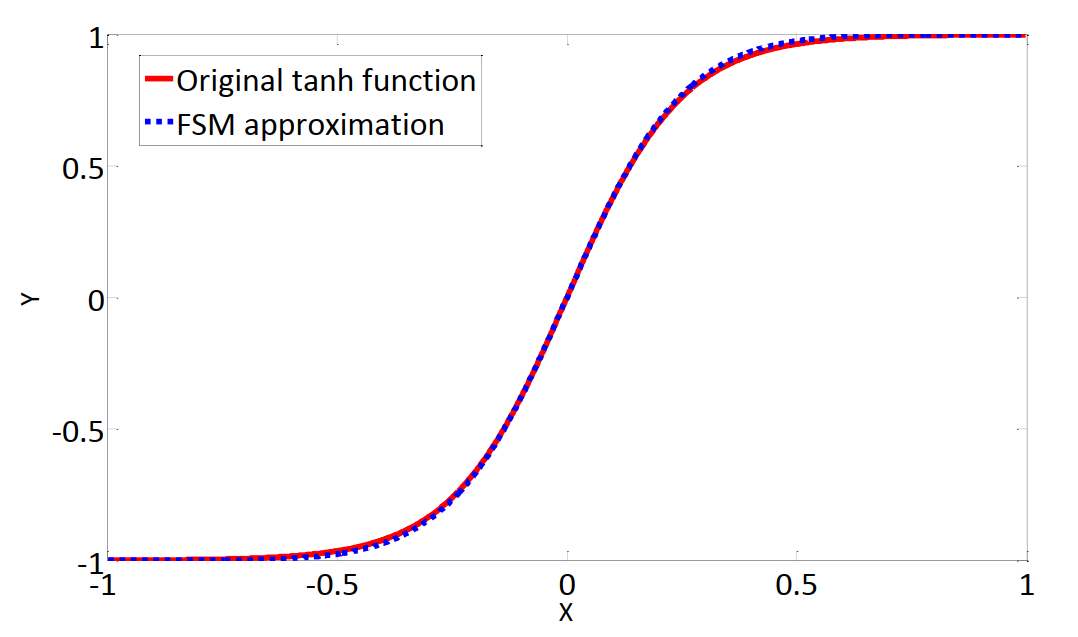
\includegraphics[width=12cm]{gfx/tanhgraph.png}
	\caption{Simulation result of the FSM-based stochastic
	tanh function}
	\label{fig:system:example1}
\end{figure}

\subsection{Stochastic Exponentiation Function (SExp)}
\begin{figure}[htb]
	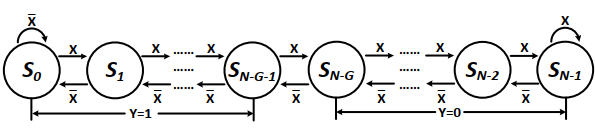
\includegraphics[width=12cm]{gfx/explsm.png}
	\caption{State transition diagram of the SAbs Function}
	\label{fig:system:example1}
\end{figure}

\subsection{Stochastic Absolute Value Function (SAbs)}


\begin{figure}[htb]
	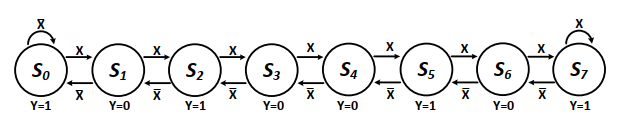
\includegraphics[width=12cm]{gfx/abslsm.png}
	\caption{State transition diagram of the SExp Function}
	\label{fig:system:example1}
\end{figure}
% !TEX root = ../my-thesis.tex
%
\chapter{Application}
\label{sec:app}


application where fault tolerance and high level of parralelization is possible. 

\section{Digital Image Processing}
\label{sec:app:sec1}

\cite{liUsingStochasticComputing2011} test

\cite{d}

\section{Multi-layer Perceptron}
\label{sec:app:sec2}


\section{Convolutional Neural Network}
\label{sec:app:sec3}



\section{Reinforcement Learning}
\label{sec:app:sec4}



% !TEX root = ../my-thesis.tex
%
\chapter{Methodology}
\label{sec:method}

\section{Cocotb \& Ikarus}
\label{sec:concepts:sec1}


\section{Xilinx Vivado}
\label{sec:concepts:sec2}


\section{Gem5}
\label{sec:concepts:sec3}


% !TEX root = ../my-thesis.tex
%
\chapter{Result}
\label{sec:result}


% !TEX root = ../my-thesis.tex
%
\chapter{Conclusion}
\label{sec:conclusion}

This thesis aims provide insights into the practicality and efficiency of SC. We intend to identify both the potential benefits and limitations of SC, determining its feasibility as an alternative to conventional digital computing. We hope to contribute to the development of more energy-efficient computing paradigms, potentially influencing future advancements in the field.
% --------------------------
% Back matter
% --------------------------
%
% \cite{Jurgens:2000,Jurgens:1995,Miede:2011,Kohm:2011,Apple:keynote:2010,Apple:numbers:2010,Apple:pages:2010}
% \cite{WEB:GNU:GPL:2010,WEB:Miede:2011}
{%
\setstretch{1.1}
\renewcommand{\bibfont}{\normalfont\small}
\setlength{\biblabelsep}{0pt}
\setlength{\bibitemsep}{0.5\baselineskip plus 0.5\baselineskip}
\printbibliography[nottype=online]
\newrefcontext[labelprefix={@}]
\printbibliography[heading=subbibliography,title={Webpages},type=online]
}
% \clearpage

% \listoffigures

% \clearpage

% \listoftables

% \clearpage

% \lstlistoflistings

% \clearpage

\appendix

% \clearpage
% % !TEX root = ../my-thesis.tex
%
\chapter{Example Appendix}
\label{sec:appendix}

\Blindtext[1][1]

\section{Appendix Section 1}
\label{sec:appendix:sec1}

\Blindtext[1][1]

\begin{table}[h]
	\begin{tabularx}{\textwidth}{X | X | X}
		%\hline
		Alpha		& Beta			& Gamma			\\ \hline
		0			& 1				& 2				\\ \hline
		3			& 4				& 5				\\ %\hline
	\end{tabularx}
	\label{tab:table1}
	\caption{This is a caption text.}
\end{table}

\section{Appendix Section 2}
\label{sec:appendix:sec2}

\Blindtext[1][1]

\begin{table}[h]
	\begin{tabularx}{\textwidth}{X | X | X}
		%\hline
		Alpha		& Beta			& Gamma			\\ \hline
		0			& 1				& 2				\\ \hline
		3			& 4				& 5				\\ %\hline
	\end{tabularx}
	\label{tab:table2}
	\caption{This is a caption text.}
\end{table}

\Blindtext[1][2]


% \clearpage
% \input{content/colophon}

% \clearpage
% % !TEX root = ../my-thesis.tex
%
%************************************************
% Declaration
%************************************************
\pdfbookmark[0]{Declaration}{Declaration}
\addchap{Declaration}
\label{sec:declaration}
\thispagestyle{empty}

You can put your declaration here, to declare that you have completed your work solely and only with the help of the references you mentioned.

\bigskip

% \noindent\textit{\thesisUniversityCity, \thesisDate}

\smallskip

\begin{flushright}
	\begin{minipage}{5cm}
		\rule{\textwidth}{1pt}
		\centering\thesisName
	\end{minipage}
\end{flushright}

%*****************************************
%*****************************************


\newpage
\mbox{}

% **************************************************
% End of Document CONTENT
% **************************************************

\end{document}
